% Part I, results of the training runs, the behaviour of the final policies, and the cost (included by main_en.tex).

\section{Training on the judges' rewards}\label{sec:results}

All \NUM{runs_total} runs finished: seven conditions on five tasks, five seeds each (three for \texttt{ar\_sampled}).
A reset of the virtual machine interrupted \NUM{resumed_runs} runs (of \NUM{resumed_conds}). They resumed from their
checkpoint at step \NUM{resumed_steps}, and each lost the episode in progress, at most \NUM{resumed_dropped_max} steps.
Table~\ref{tab:returns} gives the final returns per task, Table~\ref{tab:aggregate} the normalised aggregate, and
Figure~\ref{fig:curves} the learning curves.

\begin{table}[t]
\centering\footnotesize\setlength{\tabcolsep}{4pt}
\begin{tabular}{@{}lccccccc@{}}
\toprule
 task & \texttt{env} & \texttt{env\_window} & \texttt{kev\_score} & \texttt{kev\_gated} & \texttt{kev\_distill} & \texttt{ar\_gated} & \texttt{ar\_sampled} \\ \midrule
Hopper & 2820 $\pm$ 969 & 3419 $\pm$ 450 & 3061 $\pm$ 314 & 3169 $\pm$ 174 & 2833 $\pm$ 909 & 1165 $\pm$ 309 & 1127 $\pm$ 293 \\
Walker2d & 3150 $\pm$ 1276 & 4068 $\pm$ 1909 & 2593 $\pm$ 509 & 2536 $\pm$ 712 & 2943 $\pm$ 562 & 1321 $\pm$ 189 & 1330 $\pm$ 165 \\
HalfCheetah & 3441 $\pm$ 1152 & 2376 $\pm$ 1349 & 2845 $\pm$ 638 & 4241 $\pm$ 242 & 4117 $\pm$ 460 & 1069 $\pm$ 1046 & 1050 $\pm$ 824 \\
Swimmer & 81 $\pm$ 22 & 278 $\pm$ 104 & 99 $\pm$ 148 & 141 $\pm$ 124 & 91 $\pm$ 41 & 141 $\pm$ 120 & 118 $\pm$ 166 \\
Reacher & $-$6.4 $\pm$ 1.6 & $-$28.0 $\pm$ 9.4 & $-$48.9 $\pm$ 21.2 & $-$75.8 $\pm$ 10.9 & $-$88.4 $\pm$ 21.9 & $-$75.2 $\pm$ 21.3 & $-$68.8 $\pm$ 21.3 \\
\bottomrule
\end{tabular}

\caption{Final return per task: mean $\pm$ standard deviation over seeds of the mean return over 20 evaluation episodes
of the deterministic policy after $10^6$ steps. A uniform random policy scores \NUM{rand_hopper} (Hopper),
\NUM{rand_walker} (Walker2d), \NUM{rand_cheetah} (HalfCheetah), \NUM{rand_swimmer} (Swimmer) and \NUM{rand_reacher}
(Reacher).}
\label{tab:returns}
\end{table}

\begin{table}[t]
\centering\small
\begin{tabular}{@{}lcccccc@{}}
\toprule
condition & runs & IQM [95\% CI] & mean & median & $P(\,>\texttt{env})$ & $P(\,>\texttt{env\_window})$ \\ \midrule
\texttt{env} & 25 & 1.05 \ci{0.91}{1.16} & 1.00 & 1.03 & 0.50 & 0.46 \\
\texttt{env\_window} & 25 & 1.10 \ci{0.89}{1.26} & 1.41 & 1.21 & 0.54 & 0.50 \\
\texttt{kev\_score} & 25 & 0.78 \ci{0.60}{0.91} & 0.76 & 0.82 & 0.28 & 0.27 \\
\texttt{kev\_gated} & 25 & 1.00 \ci{0.81}{1.09} & 0.79 & 1.05 & 0.44 & 0.31 \\
\texttt{kev\_distill} & 25 & 0.98 \ci{0.82}{1.10} & 0.59 & 1.02 & 0.44 & 0.27 \\
\texttt{ar\_gated} & 25 & 0.35 \ci{0.28}{0.46} & 0.40 & 0.36 & 0.18 & 0.10 \\
\texttt{ar\_sampled} & 15 & 0.31 \ci{0.19}{0.45} & 0.37 & 0.36 & 0.12 & 0.11 \\
\bottomrule
\end{tabular}

\caption{Normalised score $(R-R_{\text{rand}})/(R_{\text{env}}-R_{\text{rand}})$ over all tasks and seeds: interquartile
mean (IQM) with a 95\% stratified-bootstrap interval, mean, median, and the probability that a run of the condition
beats a run of \texttt{env} or \texttt{env\_window} on the same task, averaged over tasks.}
\label{tab:aggregate}
\end{table}

\begin{figure}[t]
\centering
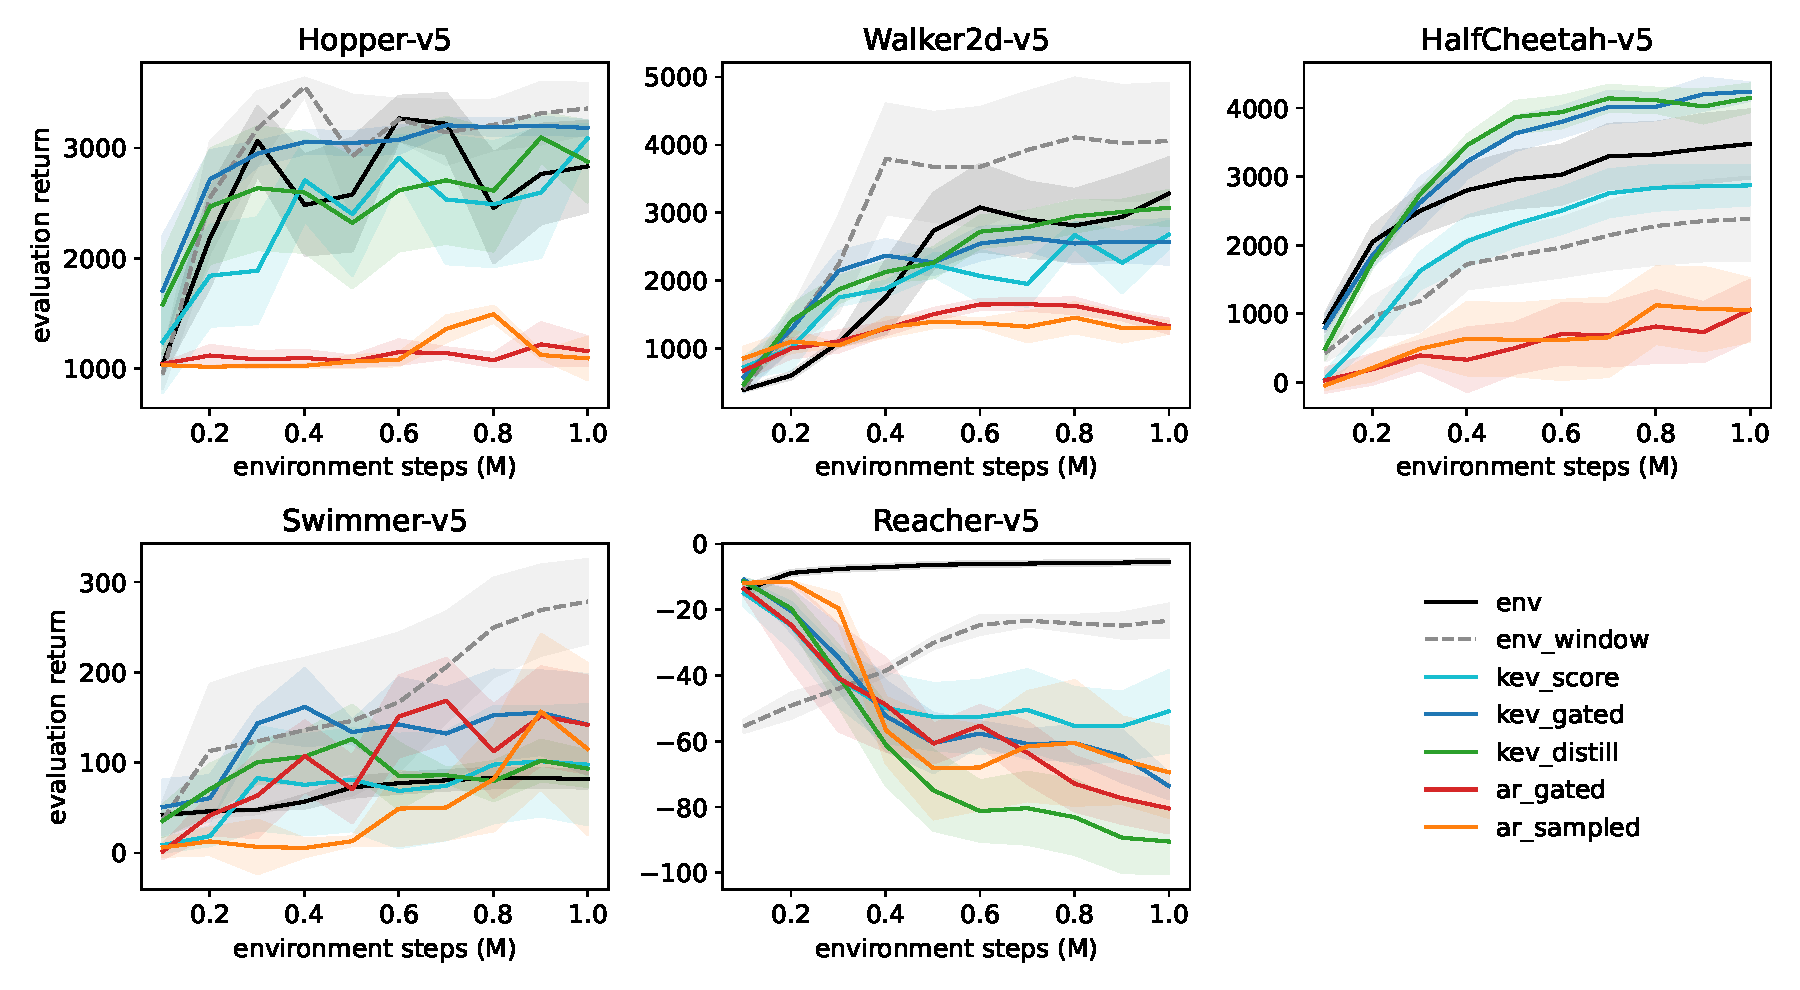
\includegraphics[width=\linewidth]{../../experiments/part1_control/results/learning_curves.pdf}
\caption{Evaluation return during training: 10 episodes every $10^5$ steps, mean over seeds, shaded $\pm$ one standard
error.}
\label{fig:curves}
\end{figure}

\paragraph{In aggregate, \kev{}'s gated and distilled rewards come close to the engineered reward, and the AR judge's
do not.}
The IQM of the normalised score is \NUM{iqm_kev_gated} \ci{\NUM{iqmlo_kev_gated}}{\NUM{iqmhi_kev_gated}} for
\texttt{kev\_gated} and \NUM{iqm_kev_distill} \ci{\NUM{iqmlo_kev_distill}}{\NUM{iqmhi_kev_distill}} for
\texttt{kev\_distill}, against \NUM{iqm_env} \ci{\NUM{iqmlo_env}}{\NUM{iqmhi_env}} for \texttt{env}. The intervals
overlap widely. A run with either reward beats a run with the engineered reward on the same task with probability
\NUM{pimpenv_kev_gated} (\texttt{kev\_gated}) and \NUM{pimpenv_kev_distill} (\texttt{kev\_distill}). Without the gate,
\kev{}'s score does worse (\NUM{iqm_kev_score} \ci{\NUM{iqmlo_kev_score}}{\NUM{iqmhi_kev_score}}, probability
\NUM{pimpenv_kev_score}). The AR judge's rewards reach about a third of the engineered reward's normalised score:
\NUM{iqm_ar_gated} \ci{\NUM{iqmlo_ar_gated}}{\NUM{iqmhi_ar_gated}} with the expected readout and \NUM{iqm_ar_sampled}
\ci{\NUM{iqmlo_ar_sampled}}{\NUM{iqmhi_ar_sampled}} with a sampled level. A \texttt{kev\_gated} run beats an
\texttt{ar\_gated} run on the same task with probability \NUM{pimp_all_kevgated_argated}. Per task this probability is
\NUM{pimp_hopper_kevgated_argated} on Hopper, \NUM{pimp_cheetah_kevgated_argated} on HalfCheetah and
\NUM{pimp_walker_kevgated_argated} on Walker2d. On Swimmer (\NUM{pimp_swimmer_kevgated_argated}) and Reacher
(\NUM{pimp_reacher_kevgated_argated}) it is close to even.

\paragraph{The aggregate hides Reacher.} The IQM leaves out the lowest and the highest quarter of the runs. The means
are lower: \NUM{mean_kev_gated} for \texttt{kev\_gated} and \NUM{mean_kev_distill} for \texttt{kev\_distill}. On Reacher
every judge's reward ends below the random policy, so these runs have negative normalised scores
(Table~\ref{tab:returns}). We therefore go through the tasks one by one.

\paragraph{Task by task.} On Hopper, \kev{}'s rewards end close to the engineered reward (\NUM{ret_hopper_kev_gated} for
\texttt{kev\_gated} against \NUM{ret_hopper_env}; probability of improvement \NUM{pimp_hopper_kevgated_env}). On Walker2d
they end lower (\NUM{ret_walker_kev_gated} for \texttt{kev\_gated} and \NUM{ret_walker_kev_distill} for
\texttt{kev\_distill}, against \NUM{ret_walker_env}; probabilities \NUM{pimp_walker_kevgated_env} and
\NUM{pimp_walker_kevdistill_env}). On HalfCheetah, \texttt{kev\_gated} (\NUM{ret_cheetah_kev_gated}) and
\texttt{kev\_distill} (\NUM{ret_cheetah_kev_distill}) end above the engineered reward (\NUM{ret_cheetah_env}; probability
\NUM{pimp_cheetah_kevgated_env} for both), for a reason we come to in \S\ref{sec:behaviour}. On Swimmer, PPO on the
engineered reward barely moves the swimmer (\NUM{ret_swimmer_env}). Every other reward does better on average, the
window-averaged true reward most (\NUM{ret_swimmer_env_window}), and the judges' rewards vary widely between seeds. On
Reacher, nothing but the engineered reward learns the task: \NUM{ret_reacher_env} with it, \NUM{ret_reacher_env_window}
with its window average, and \NUM{ret_reacher_kev_score} to \NUM{ret_reacher_kev_distill} with the judges' rewards. The
learning curves show the judges' Reacher policies getting worse as training proceeds (Figure~\ref{fig:curves}).

\paragraph{Window-level feedback costs little on locomotion and a lot on Reacher.} The true reward averaged over the
judges' windows (\texttt{env\_window}) does at least as well as the per-step reward in aggregate: IQM
\NUM{iqm_env_window} \ci{\NUM{iqmlo_env_window}}{\NUM{iqmhi_env_window}}, probability of improvement
\NUM{pimpenv_env_window}. It is ahead on Hopper (\NUM{pimp_hopper_envwindow_env}), Walker2d (\NUM{pimp_walker_envwindow_env})
and Swimmer (\NUM{pimp_swimmer_envwindow_env}). It is behind on HalfCheetah (\NUM{pimp_cheetah_envwindow_env}), where
\NUM{flipruns_cheetah_env_window} of its five runs end on their back (\S\ref{sec:behaviour}), and on Reacher
(\NUM{pimp_reacher_envwindow_env}). A Reacher episode has only two windows of 25 steps. The averaged reward no longer
tells the policy which of its actions brought the fingertip closer, and its arms end no closer to the target than a
random policy's (Table~\ref{tab:behaviour}). The judges' temporal resolution therefore explains part of their failure
on Reacher. It explains nothing of the AR judge's failure on Hopper and Walker2d, where the window-averaged reward does
well.

\paragraph{Distillation keeps \kev{}'s reward at a tenth of the judge calls.} \texttt{kev\_distill} asks the judge about
\NUM{judgewin_kev_distill} windows per run instead of \NUM{judgewin_kev_gated}, and ends level with \texttt{kev\_gated}:
IQM \NUM{iqm_kev_distill} against \NUM{iqm_kev_gated}, probability of improvement \NUM{pimp_all_kevdistill_kevgated}.
Its weakest task is Reacher (\NUM{ret_reacher_kev_distill}).

\paragraph{During training, both judges' scores track the reward to a similar degree.} For every rollout, each run
logged the correlation between the window scores it trained on and the environment's reward of the same windows. Averaged
over rollouts and runs, it is \NUM{traincorr_kev_gated} for \texttt{kev\_gated} and \NUM{traincorr_ar_gated} for
\texttt{ar\_gated}, and only \NUM{traincorr_ar_sampled} for \texttt{ar\_sampled}, whose single draws are mostly noise
(\S\ref{sec:agreement}). The two gated rewards correlate with the reward about equally, yet they train very different
policies, as the next section shows.

\subsection{What the policies learned}\label{sec:behaviour}

A return does not say what a policy does. We ran every final policy again on its 20 evaluation episodes, and recorded what
the robot did (Table~\ref{tab:behaviour}). The re-runs reproduce the logged returns exactly (largest difference
\NUM{beh_maxdiff}).

\begin{table}[t]
\centering\small
\begin{tabular}{@{}lcccccc@{}}
\toprule
 & Hopper & Walker2d & Swimmer & HalfCheetah & \multicolumn{2}{c}{Reacher} \\ \cmidrule(lr){2-2}\cmidrule(lr){3-3}\cmidrule(lr){4-4}\cmidrule(lr){5-5}\cmidrule(l){6-7}
condition & still & still & still & runs flipped & effort & distance (m) \\ \midrule
\texttt{env} & 0\% & 1\% & 62\% & 1 of 5 & 0.01 & 0.101 \\
\texttt{env\_window} & 0\% & 0\% & 14\% & 3 of 5 & 0.19 & 0.180 \\
\texttt{kev\_score} & 0\% & 4\% & 11\% & 0 of 5 & 0.36 & 0.256 \\
\texttt{kev\_gated} & 1\% & 10\% & 15\% & 0 of 5 & 0.63 & 0.263 \\
\texttt{kev\_distill} & 1\% & 1\% & 11\% & 0 of 5 & 0.76 & 0.250 \\
\texttt{ar\_gated} & 49\% & 40\% & 18\% & 0 of 5 & 0.63 & 0.253 \\
\texttt{ar\_sampled} & 26\% & 17\% & 50\% & 0 of 3 & 0.56 & 0.252 \\ \midrule
random policy & 31\% & 4\% & 26\% & -- & 0.33 & 0.180 \\
\bottomrule
\end{tabular}

\caption{Behaviour of the final policies, averaged over episodes and seeds (20 evaluation episodes per run).
\emph{still}: fraction of steps with $|v_x|<0.1$\,m/s. \emph{runs flipped}: runs whose cheetah spends more than half of
the steps on its back ($\cos(\text{pitch})<0$). \emph{effort}: mean squared action, in $[0,1]$. \emph{distance}: mean
fingertip--target distance over the episode. The random policy samples its actions uniformly.}
\label{tab:behaviour}
\end{table}

\begin{table}[t]
\centering\small
\begin{tabular}{@{}lcccccc@{}}
\toprule
 & & & \multicolumn{2}{c}{\kev{}} & \multicolumn{2}{c}{AR judge} \\ \cmidrule(lr){4-5}\cmidrule(l){6-7}
task & windows (slow / fast) & env.\ reward & progress & gated & progress & gated \\ \midrule
Hopper & 42 / 430 & 0.31 & 0.59 & 0.48 & 0.89 & 0.87 \\
Walker2d & 386 / 1238 & 0.27 & 0.62 & 0.47 & 0.90 & 0.87 \\
HalfCheetah & 309 / 1368 & $-$0.06 & 0.51 & 0.15 & 0.85 & 0.65 \\
\bottomrule
\end{tabular}

\caption{What each signal pays for standing relative to running, on the windows of \S\ref{sec:agreement} (logged by the
\texttt{env} runs). The table gives the mean over the windows without a fall that are slower than \NUM{sf_slowmax}\,m/s,
divided by the mean over those faster than \NUM{sf_fastmin}\,m/s. \emph{env.\ reward}: the per-step environment reward.}
\label{tab:slowfast}
\end{table}

\paragraph{The AR judge's reward teaches the hopper and the walker to stand.} The final \texttt{ar\_gated} policies stand
still for \NUM{still_hopper_ar_gated} of the steps on Hopper and \NUM{still_walker_ar_gated} on Walker2d. For
\texttt{kev\_gated} the figures are \NUM{still_hopper_kev_gated} and \NUM{still_walker_kev_gated}, and for \texttt{env}
\NUM{still_hopper_env} and \NUM{still_walker_env}. Their mean forward velocity is \NUM{vx_hopper_ar_gated} and
\NUM{vx_walker_ar_gated}\,m/s, against \NUM{vx_hopper_kev_gated} and \NUM{vx_walker_kev_gated}\,m/s for
\texttt{kev\_gated} and \NUM{vx_hopper_env} and \NUM{vx_walker_env}\,m/s for \texttt{env}. Their Hopper return
(\NUM{ret_hopper_ar_gated}) is close to the 1000 that the survival bonus alone pays for standing through an episode of
1000 steps. Sampling the level does not remove it: \texttt{ar\_sampled} stands still for \NUM{still_hopper_ar_sampled}
and \NUM{still_walker_ar_sampled} of the steps.

Table~\ref{tab:slowfast} shows why. It compares what each signal pays for an upright window slower than
\NUM{sf_slowmax}\,m/s with what it pays for a window faster than \NUM{sf_fastmin}\,m/s. The AR judge's gated score pays
the slow window \NUM{sfratio_hopper_argated} of the fast one on Hopper (\NUM{sfs_hopper_argated} against
\NUM{sff_hopper_argated}) and \NUM{sfratio_walker_argated} on Walker2d. The engineered reward pays
\NUM{sfratio_hopper_perstep} and \NUM{sfratio_walker_perstep}, and \kev{}'s gated score \NUM{sfratio_hopper_kevgated} and
\NUM{sfratio_walker_kevgated}. Every step of an episode receives the score of its window, and a fall ends the episode.
Under the AR judge's reward, standing upright therefore earns almost as much per step as hopping, without the risk of a
fall. PPO finds this early: the \texttt{ar\_gated} curves on Hopper are flat from the first evaluation
(Figure~\ref{fig:curves}). Yet the AR judge's scores rank the windows almost as well as \kev{}'s. Their Spearman
correlation with the reward is \NUM{rho_hopper_ar_gated} against \NUM{rho_hopper_kev_gated} on Hopper and
\NUM{rho_walker_ar_gated} against \NUM{rho_walker_kev_gated} on Walker2d (Table~\ref{tab:agreement}). What differs is the
margin: the AR judge rates almost every upright window near the top of its scale. Rank agreement with the reward did not
predict which reward PPO could use.

\paragraph{The judges' rewards keep the cheetah upright.} On HalfCheetah, \NUM{flipruns_cheetah_env} of the five
\texttt{env} runs and \NUM{flipruns_cheetah_env_window} of the five \texttt{env\_window} runs end with the cheetah on its
back. This is a local optimum that the engineered reward does not penalise. These runs return at most
\NUM{flip_maxret}, and the upright runs of the same two conditions at least \NUM{upright_minret}. None of the
\NUM{judge_runs_cheetah} runs on a judge's reward flips. The task text both judges read says that flipping is
undesirable, and the lowest \texttt{progress} level names it. Without its flipped run, \texttt{env} averages
\NUM{uprightret_env} on HalfCheetah, against \NUM{ret_cheetah_kev_gated} for \texttt{kev\_gated}, so the flip accounts for
much of \kev{}'s advantage there. Here the judge's reward carries a preference that the engineered reward leaves out, and
the policy follows it.

\paragraph{On Reacher, the judges' rewards make the arm flail.} The arms trained on a judge's reward keep the fingertip
\NUM{dist_reacher_kev_distill} to \NUM{dist_reacher_kev_gated}\,m from the target on average. That is farther than a random
policy's (\NUM{dist_reacher_random}\,m) and the engineered reward's (\NUM{dist_reacher_env}\,m). They also spend more
effort than the random policy: \NUM{effort_reacher_kev_score} to \NUM{effort_reacher_kev_distill}, against
\NUM{effort_reacher_random}, and \NUM{effort_reacher_env} for \texttt{env}. Reacher's reward charges the squared action
at every step, which is why these policies end below the random policy. Both judges' scores follow the change of the
distance within a window (Spearman \NUM{rhophys_reacher_kev_progress} for \kev{}'s and \NUM{rhophys_reacher_ar_progress}
for the AR judge's \texttt{progress}, \S\ref{sec:agreement}). They follow the distance itself, which Reacher's reward
charges at every step, much less (\NUM{rho_reacher_kev_progress} and \NUM{rho_reacher_ar_progress} with the reward).
With two windows per episode, neither signal led PPO to the target.

\section{Cost}\label{sec:cost}

\begin{table}[t]
\centering\small
\begin{tabular}{@{}lcccc@{}}
\toprule
condition & judged windows & judge wait (h) & wall-clock (h) & corr.\ (score, env reward) \\ \midrule
\texttt{env} & 0 & 0.0 & 0.1 & -- \\
\texttt{env\_window} & 0 & 0.0 & 0.1 & -- \\
\texttt{kev\_score} & 33{,}914 & 2.0 & 2.1 & 0.57 \\
\texttt{kev\_gated} & 33{,}942 & 1.9 & 2.1 & 0.56 \\
\texttt{kev\_distill} & 3{,}477 & 1.9 & 2.0 & 0.54 \\
\texttt{ar\_gated} & 33{,}861 & 1.9 & 2.0 & 0.52 \\
\texttt{ar\_sampled} & 33{,}869 & 1.9 & 2.0 & 0.17 \\
\bottomrule
\end{tabular}

\caption{Cost per run, averaged over tasks and seeds: windows sent to the judge, time spent waiting for its answers,
wall-clock time of the run, and the mean correlation, per rollout, between the window scores the run trained on and the
environment's reward of the same windows. One judge server on one GPU served up to 24 concurrent runs, so the waits include
the time it spent on the other runs' requests.}
\label{tab:cost}
\end{table}

Table~\ref{tab:cost} gives what the judges cost per run. A run that asks the judge about every window sends it about
\NUM{judgewin_kev_gated} windows over $10^6$ steps, and \texttt{kev\_distill} about \NUM{judgewin_kev_distill}. A run
without a judge took \NUM{wallh_env}\,h. A run with one took about \NUM{wallh_kev_gated}\,h, about \NUM{wallratio}
times as long, and spent nearly all of it (\NUM{waith_kev_gated}\,h) waiting for the judge. These times describe our
setup, in which one judge server on one GPU answered up to 24 runs at once. A run's wait includes the time the server
spent on the other runs' requests. That is why \texttt{kev\_distill}, with a tenth of the windows, waited about as long
(\NUM{waith_kev_distill}\,h): its requests queued behind those of the other runs. We did not measure a judge serving a
single run, which is where the distilled reward's saving would show.
